% ============================================================================
\chapter{A bancada aberta: a rodada 0.14}\label{cap:bancada}
% ============================================================================

As rodadas 0.11 e 0.12 aplicaram a separação ``uma busca propõe, um verificador decide'' a domínios escolhidos: redes de ordenação, geometria, engenharia, lógica, tabuleiros. Cada domínio era uma mesa com o seu formato de entrada e os seus exemplos. A crítica que abriu a rodada 0.14 foi direta: o módulo de ciência apresentava \emph{problemas já resolvidos}; as cenas aceitavam só ações pré-determinadas; o sistema era expositivo. Este capítulo descreve a resposta --- trocar \emph{N mesas} por \textbf{uma linguagem, uma fornalha e uma pedra de toque} --- e o que as verificações com controle disseram dela.

\begin{graduacao}
\textbf{Glossário mínimo.} Um \emph{espaço de busca} é o conjunto de candidatos possíveis (permutações, subconjuntos, grafos\ldots). Uma \emph{meta-heurística} (recozimento simulado, algoritmo evolutivo) explora esse espaço sem garantia de ótimo. Um \emph{processo gaussiano} é um modelo estatístico de uma função desconhecida, usado para escolher o próximo ponto a medir quando cada medida é cara. Um \emph{holdout} é um conjunto de dados reservado que a busca não vê, usado para descobrir se o vencedor só venceu por acaso.
\end{graduacao}

% ----------------------------------------------------------------------------
\section{Escrutínio do pedido}\label{sec:banc-escrutinio}

O pedido pedia ``uma grande coletânea'' de buscadores famosos, generalizados. Tomado ao pé da letra, isso produziria $N$ ferramentas estreitas com $N$ formatos --- exatamente a falta de liberdade criticada. O denominador comum desses buscadores é um laço de três passos: \emph{proponha} um candidato, \emph{avalie-o} com um verificador, \emph{guarde} o resultado com a prova. O produto, então, é o caso geral; os casos famosos viram \emph{exemplos de partida} escritos na mesma linguagem que o usuário usa (régua de Golomb, Ramsey, a conjectura de Euler, redes de ordenação, caixeiro-viajante, portfólios, hiperparâmetros, exemplos adversariais, regras de \textit{trading}, fórmulas). Os nomes do sistema seguem a metáfora do laboratório alquímico --- \emph{Alembic}, \emph{Athanor}, \emph{Touchstone}, \emph{Crucible}, \emph{Assay} --- e nenhum nome de produto de terceiros é usado.

Dois riscos do pedido foram tratados como requisitos. \textbf{Entrada aberta} sem sanitização é uma porta de ataque; sanitização por lista de palavras é frágil. \textbf{``AI em tudo''} sem verificação é autoridade sem prova. As duas seções seguintes mostram as respostas.

% ----------------------------------------------------------------------------
\section{Alembic: uma linguagem pura e saneada}\label{sec:banc-alembic}

Alembic é uma linguagem de expressões pura: inteiros de tamanho arbitrário, listas, tuplas, mapas, compreensões, \textit{lambdas}, \textit{pipes} e cerca de 120 funções embutidas, sem E/S, sem relógio e sem aleatoriedade fora de \code{noise} e \code{hash}, que são determinísticas. Um programa é, portanto, uma função do seu texto --- o que torna reprodutível o diário de toda busca que o use.

A sanitização é feita pela \emph{semântica}, não por filtros (\autoref{tab:banc-limites}): todo passo paga combustível; tamanhos têm teto; a avaliação roda num processo com teto de memória que a máquina virtual mata; identificadores nunca viram átomos (a tabela de átomos da BEAM não é coletada); dados são lidos por um leitor que recusa código; e, no navegador, as expressões das cenas são uma árvore JSON \emph{interpretada}, nunca avaliada como JavaScript. A mesma análise achou um vazamento antigo: \code{Vapor.Expr.compile/2} criava um módulo BEAM (e um átomo) por expressão nova; agora há um teto, e o excedente é interpretado sem criar átomo algum.

\begin{table}[htbp]
\centering
\caption{Os limites da Alembic e o teste que tenta quebrar cada um}\label{tab:banc-limites}
\small
\begin{tabularx}{\textwidth}{@{}l>{\raggedright\arraybackslash}X>{\raggedright\arraybackslash}X@{}}
\toprule
\textbf{risco} & \textbf{defesa} & \textbf{teste}\\
\midrule
laço infinito & combustível em toda chamada e iteração & recursão sem fim e \code{fold} gigante recusados\\
números enormes & inteiros até 65\,536 bits & $2^{10^8}$ recusado\\
memória & processo com \code{max\_heap\_size} & bomba de memória morta sob 16 MB; o chamador vive\\
átomos & identificadores ficam binários & 2\,000 nomes novos: 0 átomos\\
código como dado & leitor de literais & \code{f(1)} e compreensões recusados\\
injeção no navegador & árvore interpretada & funções não numéricas recusadas\\
\bottomrule
\end{tabularx}
\end{table}

% ----------------------------------------------------------------------------
\section{Athanor e Touchstone}\label{sec:banc-athanor}

Um problema Athanor é um programa Alembic com nomes reservados: \code{space} (dez construtores: \code{bits}, \code{ints}, \code{reals}, \code{perm}, \code{subset}, \code{subsets}, \code{seq}, \code{graph}, \code{partition} e \code{program}, árvores de expressão), um objetivo (\code{minimize}, \code{maximize}) ou uma afirmação (\code{claim}), e opcionalmente \code{violation} (a distância até a validade, que ordena os inválidos e deixa a busca subir até eles), \code{holdout}, \code{describe} (para um arquivo MAP-Elites), \code{neighbor} e \code{measured}.

A fornalha reparte o orçamento entre estratégias --- exaustiva retomável, aleatória, recozimento, evolução, CMA-ES, otimização bayesiana com processo gaussiano Matérn-5/2, \emph{mente} (um modelo de linguagem) e \emph{humano} --- por um bandido UCB descontado ($\gamma = 0{,}97$). A primeira versão, com UCB simples, gastava demais na aleatória; sem a aleatória, perdia nos problemas rugosos; o desconto resolveu os dois. Toda corrida termina com três objetos que a tornam julgável:
\begin{enumerate}
  \item o \textbf{controle}: o mesmo orçamento gasto em amostras uniformes; se o acaso nunca alcança o melhor, a regra de três dá o limite superior da chance por amostra;
  \item o \textbf{\textit{holdout}}: os finalistas reavaliados num objetivo não visto, com a correlação de postos de Spearman e o máximo esperado do ruído, $\sqrt{2 \ln N}$;
  \item o \textbf{diário}: uma cadeia SHA-256 sobre a codificação canônica de cada avaliação, cuja raiz depende só do texto e da semente.
\end{enumerate}

A \textbf{Touchstone} reconfere um certificado sem confiar na busca: reavalia o candidato, confere pertença e valor; com \code{full}, refaz a enumeração; com \code{replay}, refaz a corrida e compara a raiz do diário. ``Provado'' significa exatamente \emph{enumeração completa de um espaço finito}, e o certificado diz o tamanho.

\paragraph{Humano e modelo no laço.} Uma sessão corre sob supervisão; a pessoa observa, propõe candidatos, fixa e bane finalistas, estende o orçamento ou fornece medidas de um objetivo externo (um experimento, um treino). Um modelo de linguagem pode \emph{formalizar} um problema descrito em palavras --- o rascunho é compilado, reparado até três vezes com o erro do compilador e devolvido com uma \emph{retrotradução} para a pessoa conferir --- e pode \emph{propor} candidatos. As propostas, venham de onde vierem, entram pela mesma porta e são julgadas pelo mesmo verificador. O modelo nunca decide.

% ----------------------------------------------------------------------------
\section{Crucible: evidência sem gabarito}\label{sec:banc-crucible}

Os experimentos científicos das rodadas anteriores comparavam a saída com uma resposta conhecida --- útil como calibração, inútil para quem traz um sistema novo, cuja resposta ninguém conhece. O Crucible aceita o sistema do usuário (EDOs, potenciais, hamiltonianos, reações, sequências, moléculas, dados) e responde com evidência que \emph{não precisa de gabarito}: a ordem de convergência observada por Richardson; teoremas que valem para qualquer entrada (virial, Ehrenfest, trabalho--energia); dois métodos independentes que precisam concordar; e controles que um método errado reprovaria.

O caso mais forte são as \textbf{leis de conservação provadas sobre $\mathbb{Q}$}. Para um campo vetorial polinomial, um candidato $I = \sum_k c_k m_k$ (monômios e, opcionalmente, logaritmos das variáveis) é conservado se e só se a derivada de Lie $\sum_i f_i \,\partial I/\partial x_i$ se anula identicamente; isso é um sistema linear nos $c_k$, resolvido exatamente em racionais. Para a epidemia SIR, o método acha $S + I + R$ e $3S + 3I - \ln S$, ambos provados, e mostra que sobrevivem a perturbar cada coeficiente em 1\,\% (são estruturais). Na verificação com controle (\autoref{tab:qualidade14}), seis hamiltonianos cúbicos aleatórios têm o seu $H$ redescoberto e provado, e seis sistemas dissipativos aleatórios não recebem lei nenhuma.

% ----------------------------------------------------------------------------
\section{Assay: essa diferença é real?}\label{sec:banc-assay}

Voltando às raízes do projeto em pesquisa de IA, o Assay ataca a dor mais comum do campo, que não é treinar, mas \emph{decidir se uma diferença de avaliação é real}: comparação pareada com \textit{bootstrap}, permutação por troca de sinal e McNemar exato, junto do efeito mínimo detectável; \textit{leaderboards} com empates declarados; calibração medida contra o seu próprio piso (o ECE que um modelo perfeitamente calibrado teria com aquelas confianças e aquele $n$); concordância de anotadores (Krippendorff, Fleiss, Cohen); viés de posição de juízes; contaminação por 13-gramas; deduplicação por MinHash verificada por Jaccard exato; e leis de escala na forma de Hoffmann, que precisam \emph{prever as maiores corridas sem tê-las visto}.

O controle da lei de escala --- as mesmas corridas com as perdas embaralhadas --- achou um defeito real: sem estrutura nos dados, os parâmetros em escala logarítmica cresciam até estourar a exponencial. O ajuste agora permanece finito, e o \textit{holdout} reporta erro de 33\,\% contra 0,3\,\% com os dados verdadeiros: a lei não prevê nada, que é a resposta certa.

% ----------------------------------------------------------------------------
\section{Interfaces: o terminal primeiro}\label{sec:banc-interfaces}

Toda capacidade da bancada está disponível na linha de comando (\code{bin/vapor}), na filosofia Unix: leitura da entrada padrão, JSON quando a saída é um \textit{pipe}, e códigos de saída com significado (0 positivo, 1 negativo --- refutado, não achado, verificação falhou, ruído ---, 2 uso, 3 entrada inválida, 4 falha). O console web, a TUI e as 20 ferramentas MCP chamam as mesmas funções. O console ganhou uma identidade visual própria em que o ornamento coincide com a informação: a \emph{fornalha} é o gráfico ao vivo da busca (faíscas por avaliação, a linha do melhor, a linha tracejada do controle, a partilha do portfólio) e a \emph{pedra de toque} é o veredito, um risco de ouro por verificação aprovada e de chumbo pela reprovada (\autoref{fig:banc-console}). As cenas passaram a ser documentos editados por operações de texto, com expressões por quadro e direção por modelo.

\begin{figure}[htbp]
\centering
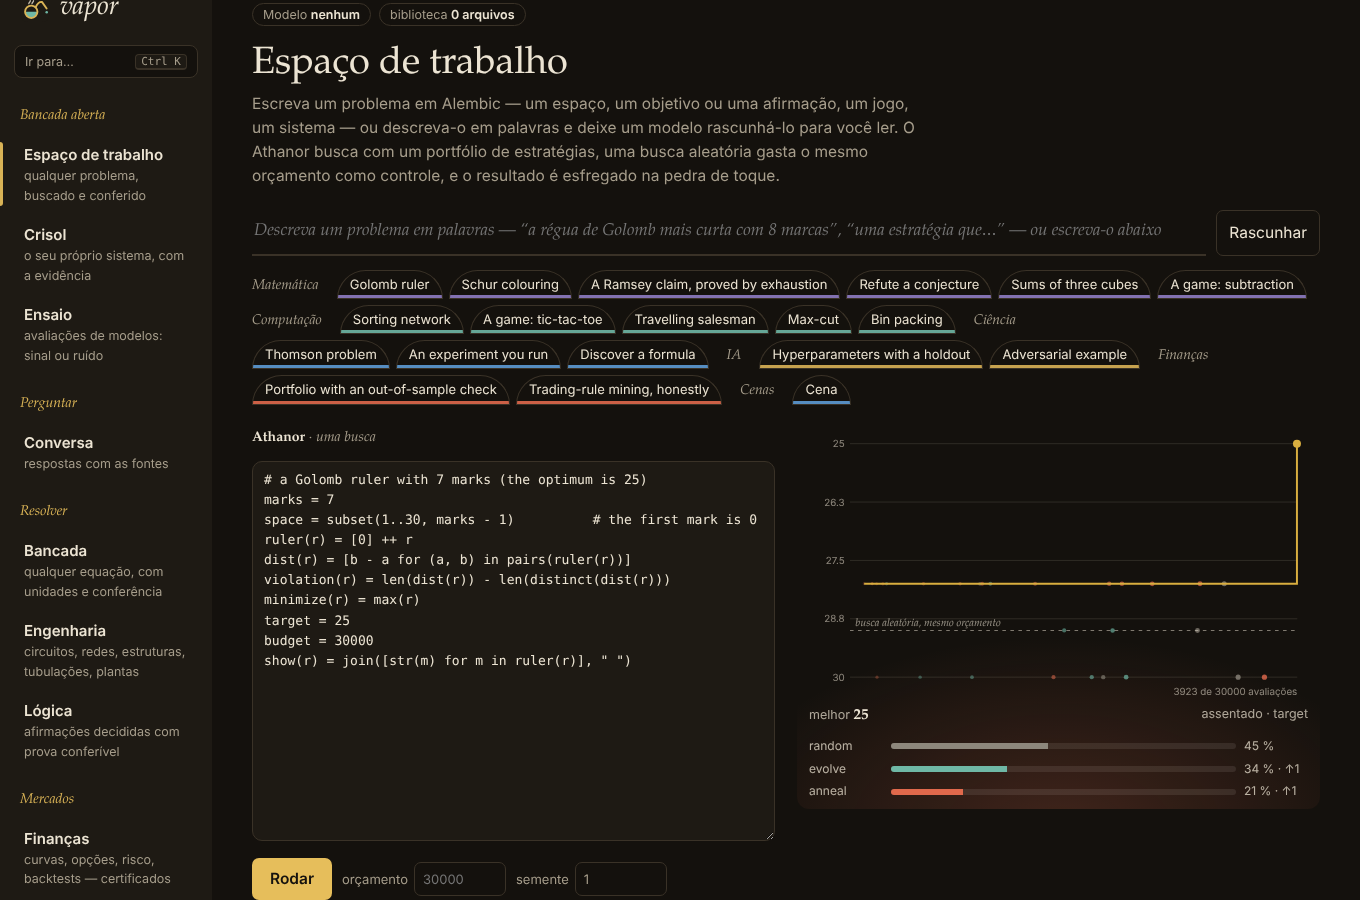
\includegraphics[width=0.9\textwidth]{../docs/img/bancada-athanor-escuro.png}
\caption{O espaço de trabalho: a régua de Golomb de 7 marcas achada no ótimo (25); a linha tracejada é a busca aleatória com o mesmo orçamento, que não passou de 28; abaixo, a partilha do portfólio.}
\label{fig:banc-console}
\end{figure}

% ----------------------------------------------------------------------------
\section{O que este capítulo não afirma}\label{sec:banc-limites}

\begin{itemize}
  \item Que ``provado'' signifique mais que enumeração completa de um espaço finito; espaços infinitos dão evidência, e o certificado diz qual.
  \item Que a fornalha seja competitiva com resolvedores especializados (SAT, MIP) nos seus domínios --- as mesas exatas de lógica e de programação linear continuam existindo.
  \item Que o rascunho de um modelo esteja certo: a retrotradução existe para que a pessoa confira.
  \item Química além de STO-3G de camada fechada com H e He.
\end{itemize}
